\documentclass[10pt,a4paper]{article}
\usepackage[T1]{fontenc}
\usepackage{lmodern}
\usepackage{amsmath,amssymb,array,booktabs,longtable,tabularx,graphicx,float,placeins}
\usepackage[margin=20mm]{geometry}
\usepackage[unicode,colorlinks=true,linkcolor=blue,urlcolor=blue]{hyperref}
\newcolumntype{P}[1]{>{\raggedright\arraybackslash}p{#1}}
\setlength{\parindent}{0pt}
\setlength{\parskip}{5pt}
\setlength{\emergencystretch}{3em}
\setlength{\tabcolsep}{4pt}
\renewcommand{\arraystretch}{1.18}

\title{Numerical Experiments}
\author{}
\date{}
\begin{document}
\maketitle

\begingroup\sloppy
\section{Overview}

This document specifies the experimental design, execution, and results used to check consistency between the mathematical model and its implementation and to analyze parameter sensitivity. The model is specified in \texttt{1. B.baseline\_model/1)baseline/baseline(main).tex}.

The implementation is first verified using a small instance. Further experiments will then use parameter values derived from observations. Sensitivity is examined separately for each parameter.

\par\endgroup

\section{Small Synthetic Instance: Model Verification and Sensitivity Analysis}
\label{sec:smallcase}
\textbf{Purpose.} Verify agreement between the formulation and the code using a small synthetic instance that can be checked directly. Vary the inputs to identify ranges of stable optimal allocations, switching points, and changes in throughput and cost.

\subsection{Baseline Experiment}
\subsubsection{Inputs and Common Settings}
The values in Table~\ref{tab:sc-input} are synthetic inputs chosen for implementation verification. Only market size $M_c$ differs across cities; costs, vehicle productivity, and vehicle limits are identical.
\begin{table}[H]
\centering\small
\caption{Baseline Inputs by City}\label{tab:sc-input}
\begin{tabular}{llrrr}
\toprule
Parameter & Definition and unit & A & B & C\\\midrule
$M_c$ & Potential trip opportunities (trips/year) & 80 & 100 & 120\\
$\kappa_c$ & Service capacity (trips/vehicle/year) & 10 & 10 & 10\\
$\bar q_c$ & City-specific vehicle limit (vehicles) & 2 & 2 & 2\\
$F_c$ & Initial entry cost (USD/city) & 20 & 20 & 20\\
$K_c$ & Fixed vehicle cost (USD/vehicle/year) & 5 & 5 & 5\\
$c_c^+$ & Unused-capacity penalty (USD/trip) & 0 & 0 & 0\\
$c_c^-$ & Forgone contribution margin (USD/trip) & 10 & 10 & 10\\
\bottomrule
\end{tabular}
\end{table}
\begin{table}[H]
\centering\small
\caption{Common Settings}\label{tab:sc-common}
\begin{tabular}{P{.19\linewidth}P{.72\linewidth}}
\toprule
Item & Setting\\\midrule
$C,Q$ & $C=\{A,B,C\}$, total fleet limit $Q=4$ vehicles\\
$S$ & $|S|=10$, probability of each scenario $1/|S|=0.1$\\
$D_c^s$ & $D_c^s=M_cp_c^s$; $p_c^s$ is a manually specified choice probability (0.05, 0.2, 0.5, 0.8)\\
Evaluation period & One year after entry: one-time entry cost plus costs and losses for that year\\
$y_c,q_c$ & $y_c,q_c$ are chosen before observing demand and apply to every scenario\\
Operations & No vehicle relocation or capacity sharing across cities; demand in cities not entered is also counted as unmet\\
Verification & SciPy MILP (HiGHS) compared with independent enumeration; no random sampling\\
\bottomrule
\end{tabular}
\end{table}
The choice probability $p_c^s$ differs from the scenario occurrence probability $1/|S|$. Each row represents one joint demand scenario, not a step in a time sequence. The mean choice probability is $0.38$ in every city, and the marginal distributions are identical.
\begin{table}[H]
\centering\small
\caption{Manually Designed Choice Probabilities and Demand Scenarios}\label{tab:sc-scenarios}
\begin{tabular}{lrrrrrr}
\toprule
$s$ & $p_A^s$ & $p_B^s$ & $p_C^s$ & $D_A^s$ & $D_B^s$ & $D_C^s$\\\midrule
1 & 0.05 & 0.05 & 0.05 & 4 & 5 & 6\\
2 & 0.2 & 0.2 & 0.2 & 16 & 20 & 24\\
3 & 0.5 & 0.5 & 0.5 & 40 & 50 & 60\\
4 & 0.8 & 0.8 & 0.8 & 64 & 80 & 96\\
5 & 0.05 & 0.2 & 0.5 & 4 & 20 & 60\\
6 & 0.2 & 0.5 & 0.05 & 16 & 50 & 6\\
7 & 0.5 & 0.05 & 0.2 & 40 & 5 & 24\\
8 & 0.2 & 0.5 & 0.8 & 16 & 50 & 96\\
9 & 0.5 & 0.8 & 0.2 & 40 & 80 & 24\\
10 & 0.8 & 0.2 & 0.5 & 64 & 20 & 60\\
Mean & 0.38 & 0.38 & 0.38 & 30.4 & 38 & 45.6\\
\bottomrule
\end{tabular}
\end{table}

\subsubsection{Calculation of Performance Metrics}
For each city and scenario, served demand, unmet demand, and unused capacity are defined as follows.
\[
T_c^s=\min(D_c^s,\kappa_cq_c),\quad
U_c^s=\max(D_c^s-\kappa_cq_c,0),\quad
O_c^s=\max(\kappa_cq_c-D_c^s,0).
\]
Averages are arithmetic means over the ten scenarios. \textbf{The service rate is calculated across all candidate cities}.
\[
\mathrm{SR}\;(\%)=
\frac{\frac{1}{|S|}\sum_{s\in S}\sum_{c\in C}T_c^s}
{\frac{1}{|S|}\sum_{s\in S}\sum_{c\in C}D_c^s}\times100,
\qquad
\mathrm{CU}\;(\%)=
\frac{\frac{1}{|S|}\sum_{s\in S}\sum_{c\in C}T_c^s}{\sum_{c\in C}\kappa_cq_c}\times100.
\]
A ratio is undefined when its denominator is zero. \textbf{Utilization measures the fraction of service capacity used}, not the fraction of time vehicles are operating. The objective and improvement relative to no entry are defined below.
\begin{align*}
Z(y,q)&=\sum_{c\in C}F_cy_c+\sum_{c\in C}K_cq_c
+\frac{1}{|S|}\sum_{s\in S}\sum_{c\in C}(c_c^+O_c^s+c_c^-U_c^s),\\
Z_0&=\frac{1}{|S|}\sum_{s\in S}\sum_{c\in C}c_c^-D_c^s,\\
\Delta Z&=Z_0-Z(y,q).
\end{align*}
The improvement measures the benefit relative to no entry under the same inputs. The objective includes forgone contribution margin and therefore does not equal actual cash expenditure.

\paragraph{Notation used in tables and figures.}
For $X\in\{D,T,U,O\}$, define the city-level scenario mean
$\bar X_c=|S|^{-1}\sum_sX_c^s$ and its total $\bar X=\sum_c\bar X_c$.
Thus $\bar T$, $\bar U$, and $\bar O$ denote expected served demand, unmet demand, and unused capacity.
$\mathrm{SR}$ is the service rate and $\mathrm{CU}$ is capacity utilization, both expressed as percentages.
For compact cost headers, use
\[
C_F=\sum_cF_cy_c,\quad C_K=\sum_cK_cq_c,\quad
C_O=\frac{1}{|S|}\sum_{s,c}c_c^+O_c^s,\quad
C_U=\frac{1}{|S|}\sum_{s,c}c_c^-U_c^s.
\]
Hence $Z=C_F+C_K+C_O+C_U$ and $\Delta Z=Z_0-Z$.
$q^{\mathrm{rep}}$ denotes the representative optimal allocation and $Z^*$ the optimal scenario-based objective.
All allocation vectors list cities in the order $(A,B,C)$.

\subsubsection{Optimal Allocation and Cost}
The optimal solution is $y=(0,1,1)$ and $q=(0,2,2)$. Independent enumeration of all 60 feasible $(y,q)$ pairs gives the same result, and the baseline optimum is unique. All checks passed: integrality, nonnegativity, city-specific and total fleet limits, demand--capacity balance, and objective recalculation.
\begin{table}[H]
\centering\small
\caption{City-Level Results for the Baseline Optimum (Trips/Year)}\label{tab:sc-base-city}
\begin{tabular}{lrrrrrrr}
\toprule
$c$ & $y_c$ & $q_c$ & $\kappa_cq_c$ & $\bar D_c$ & $\bar T_c$ & $\bar U_c$ & $\bar O_c$\\\midrule
A & 0 & 0 & 0 & 30.4 & 0 & 30.4 & 0\\
B & 1 & 2 & 20 & 38 & 17 & 21 & 3\\
C & 1 & 2 & 20 & 45.6 & 17.2 & 28.4 & 2.8\\
Total & 2 & 4 & 40 & 114 & 34.2 & 79.8 & 5.8\\
\bottomrule
\end{tabular}
\end{table}
\begin{table}[H]
\centering\small
\caption{Baseline Cost Breakdown and Performance (USD)}\label{tab:sc-base-cost}
\begin{tabular}{rrrrrrr}
\toprule
$C_F$ & $C_K$ & $C_O$ & $C_U$ & $Z$ & $Z_0$ & $\Delta Z$\\\midrule
40 & 20 & 0 & 798 & 858 & 1,140 & 282\\
\bottomrule
\end{tabular}
\end{table}
The service rate is $34.2/114=30.0\%$, and capacity utilization is $34.2/40=85.5\%$. The capacity of 40 trips is not always fully used. Unused capacity in a low-demand city cannot be transferred to another city, leaving an average of 5.8 trips of unused capacity. Subtracting entry costs of 40 and vehicle costs of 20 from the service contribution margin of $34.2\times10=342$ gives an improvement of 282.
\begin{table}[H]
\centering\small
\caption{Scenario Totals for Allocation $(0,2,2)$ (Trips/Year)}\label{tab:sc-scenario-result}
\begin{tabular}{lrrrr}
\toprule
$s$ & $\sum_c D_c^s$ & $\sum_c T_c^s$ & $\sum_c U_c^s$ & $\sum_c O_c^s$\\\midrule
1 & 15 & 11 & 4 & 29\\
2 & 60 & 40 & 20 & 0\\
3 & 150 & 40 & 110 & 0\\
4 & 240 & 40 & 200 & 0\\
5 & 84 & 40 & 44 & 0\\
6 & 72 & 26 & 46 & 14\\
7 & 69 & 25 & 44 & 15\\
8 & 162 & 40 & 122 & 0\\
9 & 144 & 40 & 104 & 0\\
10 & 144 & 40 & 104 & 0\\
Total & 1,140 & 342 & 798 & 58\\
Mean & 114 & 34.2 & 79.8 & 5.8\\
\bottomrule
\end{tabular}
\end{table}
\subsubsection{Why Concentrate in B and C?}
Comparing the six allocations that use the same four vehicles separates the effects of city selection and entry costs. The optimization also considers allocations using zero to three vehicles, not just these six alternatives.
\begin{table}[H]
\centering\small
\caption{Comparison of All Four-Vehicle Allocations (Costs in USD)}\label{tab:sc-six}
\begin{tabular}{lrrrrr}
\toprule
$q$ & $\bar T$ & $C_F$ & $C_K$ & $C_U$ & $Z$\\\midrule
$(0,2,2)$ & 34.2 & 40 & 20 & 798 & 858\\
$(1,1,2)$ & 35 & 60 & 20 & 790 & 870\\
$(1,2,1)$ & 35 & 60 & 20 & 790 & 870\\
$(2,0,2)$ & 32.8 & 40 & 20 & 812 & 872\\
$(2,2,0)$ & 32.6 & 40 & 20 & 814 & 874\\
$(2,1,1)$ & 33.8 & 60 & 20 & 802 & 882\\
\bottomrule
\end{tabular}
\end{table}
\begin{figure}[H]
\centering
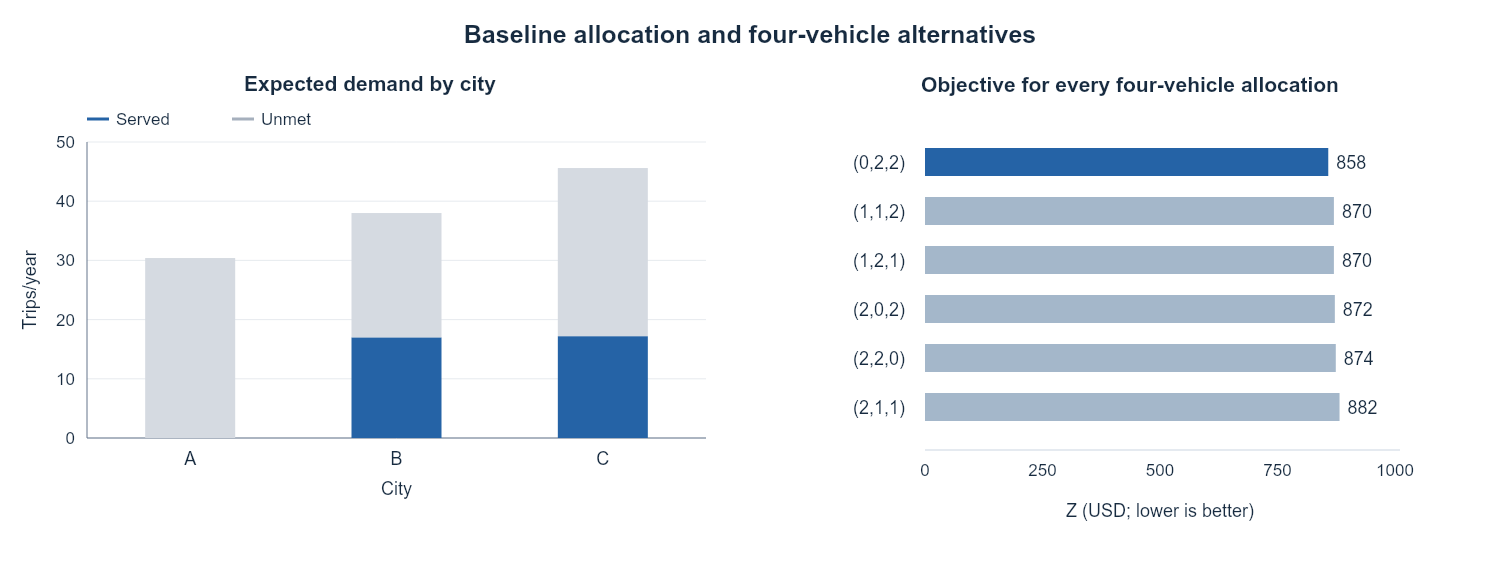
\includegraphics[width=\linewidth]{figures/smallcase/01_baseline.png}
\caption{Served and unmet demand by city, and objective values for four-vehicle allocations.}\label{fig:sc-01_baseline}
\end{figure}
\textbf{Interpretation.} With other city-specific conditions held equal in this instance, selecting the larger markets B and C is advantageous. Capacity limits prevent throughput from increasing in proportion to market size. Allocations $(1,1,2)$ and $(1,2,1)$ serve 0.8 more trips than $(0,2,2)$, but the additional entry cost of 20 exceeds the additional contribution margin of 8, increasing the objective by 12.

\FloatBarrier
\subsection{Edge-Case Experiments}
Edge cases test whether the model behaves as expected when vehicles or demand are absent, or costs take extreme values. Each experiment changes only the listed input relative to the baseline. Solutions were compared with independent enumeration, and predefined expected properties were checked for all optimal solutions.
\begin{table}[H]
\centering\small
\caption{Modified Inputs and Expected Properties for Edge Cases}\label{tab:sc-edge-design}
\begin{tabular}{lP{.36\linewidth}P{.47\linewidth}}
\toprule
Case & Modified input & Expected property\\\midrule
E1 & $Q=0$ & $y=q=0$; $U_c^s=D_c^s$\\
E2 & $M=(0,0,0)$ & $y=q=0$; $Z=0$, $U_c^s=O_c^s=0$\\
E3 & $\bar q=(0,2,2)$ & $y_A=q_A=0$\\
E4 & $c^-=(0,0,0)$ & No service incentive: $y=q=0$, $Z=0$\\
E5 & $F=(10000,10000,10000)$ & Entry costs prohibitively high: $y=q=0$\\
E6 & $Q=8$ & City limits reached: $q=(2,2,2)$, $\sum_cq_c=6$\\
E7 & $F=(0,0,0)$ & $q_c>0\implies y_c=1$\\
E8 & $p_c^s=10/M_c$ ($\forall c,s$) & $D_c^s=10$; $q=(1,1,1)$; $U_c^s=O_c^s=0$\\
\bottomrule
\end{tabular}
\end{table}
\begin{table}[H]
\centering\small
\caption{Allocation and Service Results for Edge Cases}\label{tab:sc-edge-service}
\begin{tabular}{lrrrrrr}
\toprule
Case & $q^{\mathrm{rep}}$ & $\bar T$ & $\mathrm{SR}$ (\%) & $\bar U$ & $\bar O$ & Check\\\midrule
E1 & $(0,0,0)$ & 0 & 0 & 114 & 0 & PASS\\
E2 & $(0,0,0)$ & 0 & --- & 0 & 0 & PASS\\
E3 & $(0,2,2)$ & 34.2 & 30 & 79.8 & 5.8 & PASS\\
E4 & $(0,0,0)$ & 0 & 0 & 114 & 0 & PASS\\
E5 & $(0,0,0)$ & 0 & 0 & 114 & 0 & PASS\\
E6 & $(2,2,2)$ & 49.8 & 43.68 & 64.2 & 10.2 & PASS\\
E7 & $(1,1,2)$ & 35 & 30.7 & 79 & 5 & PASS\\
E8 & $(1,1,1)$ & 30 & 100 & 0 & 0 & PASS\\
\bottomrule
\end{tabular}
\end{table}
\begin{table}[H]
\centering\small
\caption{Edge-Case Cost Breakdown and Improvement (USD)}\label{tab:sc-edge-cost}
\begin{tabular}{lrrrrrrr}
\toprule
Case & $C_F$ & $C_K$ & $C_O$ & $C_U$ & $Z$ & $Z_0$ & $\Delta Z$\\\midrule
E1 & 0 & 0 & 0 & 1,140 & 1,140 & 1,140 & 0\\
E2 & 0 & 0 & 0 & 0 & 0 & 0 & 0\\
E3 & 40 & 20 & 0 & 798 & 858 & 1,140 & 282\\
E4 & 0 & 0 & 0 & 0 & 0 & 0 & 0\\
E5 & 0 & 0 & 0 & 1,140 & 1,140 & 1,140 & 0\\
E6 & 60 & 30 & 0 & 642 & 732 & 1,140 & 408\\
E7 & 0 & 20 & 0 & 790 & 810 & 1,140 & 330\\
E8 & 60 & 15 & 0 & 0 & 75 & 300 & 225\\
\bottomrule
\end{tabular}
\end{table}
\begin{figure}[H]
\centering
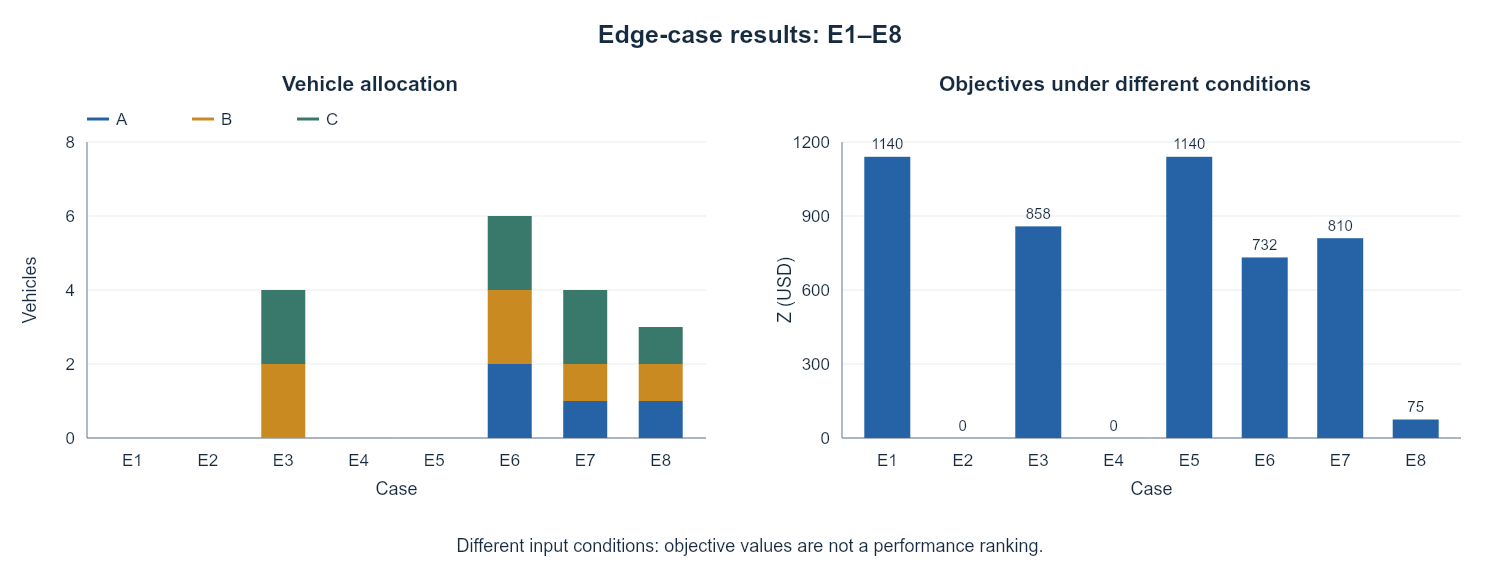
\includegraphics[width=\linewidth]{figures/smallcase/04_edges.png}
\caption{Allocations and objectives for E1--E8. Objectives under different conditions do not constitute a performance ranking.}\label{fig:sc-04_edges}
\end{figure}
\textbf{Interpretation.} E1, E4, and E5 all result in no entry, but E4 has a zero objective because the unmet-demand loss coefficient is zero. E6 deploys only six vehicles despite a total limit of eight because of the city-specific limits. E7 has two optimal allocations: $(1,1,2)$ and $(1,2,1)$. E8 serves all demand with one vehicle per city, leaving the fourth vehicle unused. The service rate in E2 is undefined because demand is zero. Even when $c^+=c^-=0$, reported unmet demand and unused capacity were recalculated from the difference between demand and capacity.

\FloatBarrier
\subsection{Sensitivity Analysis}
\subsubsection{Experimental Design and Interpretation}
One input type is varied at a time, with all other inputs fixed at their baseline values, and the model is reoptimized. Both allocation changes and performance changes are examined. Experiments that change costs or productivity jointly across cities vary a common level, whereas the $M_A$ experiment changes only A's relative market size.
\begin{table}[H]
\centering\small
\caption{Parameter Ranges for the Main Sensitivity Experiments}\label{tab:sc-sensitivity-design}
\begin{tabular}{lP{.48\linewidth}P{.35\linewidth}}
\toprule
Parameter & Variation and range & Fixed inputs\\\midrule
$Q$ & Total fleet limit: 0--8, step 1 & $\bar q_c=2$; all other inputs at baseline\\
$F$ & Common across cities: 0--20, step 1; additional higher values & Vehicle costs, demand, and other inputs at baseline\\
$\kappa$ & Common across cities: 5--20, step 0.5 & $Q=4$, $c^+=0$; other inputs at baseline\\
$M_A$ & A only: 0.5--2 times baseline, step 0.05 & $M_B,M_C$, all $p_c^s$, and other inputs at baseline\\
$c^+$ & Common across cities: 0--20, step 0.5 & Unmet-demand loss, demand, and other inputs at baseline\\
$\alpha$ & Demand variability multiplier: 0--1, step 0.05 & City mean demands and number of scenarios unchanged\\
\bottomrule
\end{tabular}
\end{table}
Additional tested values of $F$ are $40,80,120,150,155,159,160,161,162,163,170,200$. Read the panels in this order: allocation, service rate, cost breakdown, and improvement over no entry. Shaded bands show the range across tied optimal solutions, not confidence intervals. A representative solution is selected by first minimizing the number of entered cities, then using lexicographic order on $q$ and $y$. Costs can change even when the allocation remains unchanged. In particular, changing $M$ or $c^-$ also changes the comparison benchmark, so the objective alone should not be used to rank performance.

\subsubsection{Total Fleet Limit $Q$}
\begin{table}[H]
\centering\small
\caption{Selected Results: Total Fleet Limit (Throughput in Trips/Year; Costs in USD)}\label{tab:sc-selected-Q}
\begin{tabular}{lrrrrr}
\toprule
Value & $q^{\mathrm{rep}}$ & $\bar T$ & $\mathrm{SR}$ (\%) & $Z$ & $\Delta Z$\\\midrule
0 & $(0,0,0)$ & 0 & 0 & 1,140 & 0\\
3 & $(0,1,2)$ & 26.2 & 22.98 & 933 & 207\\
4 & $(0,2,2)$ & 34.2 & 30 & 858 & 282\\
5 & $(1,2,2)$ & 43 & 37.72 & 795 & 345\\
6 & $(2,2,2)$ & 49.8 & 43.68 & 732 & 408\\
8 & $(2,2,2)$ & 49.8 & 43.68 & 732 & 408\\
\bottomrule
\end{tabular}
\end{table}
\begin{figure}[H]
\centering
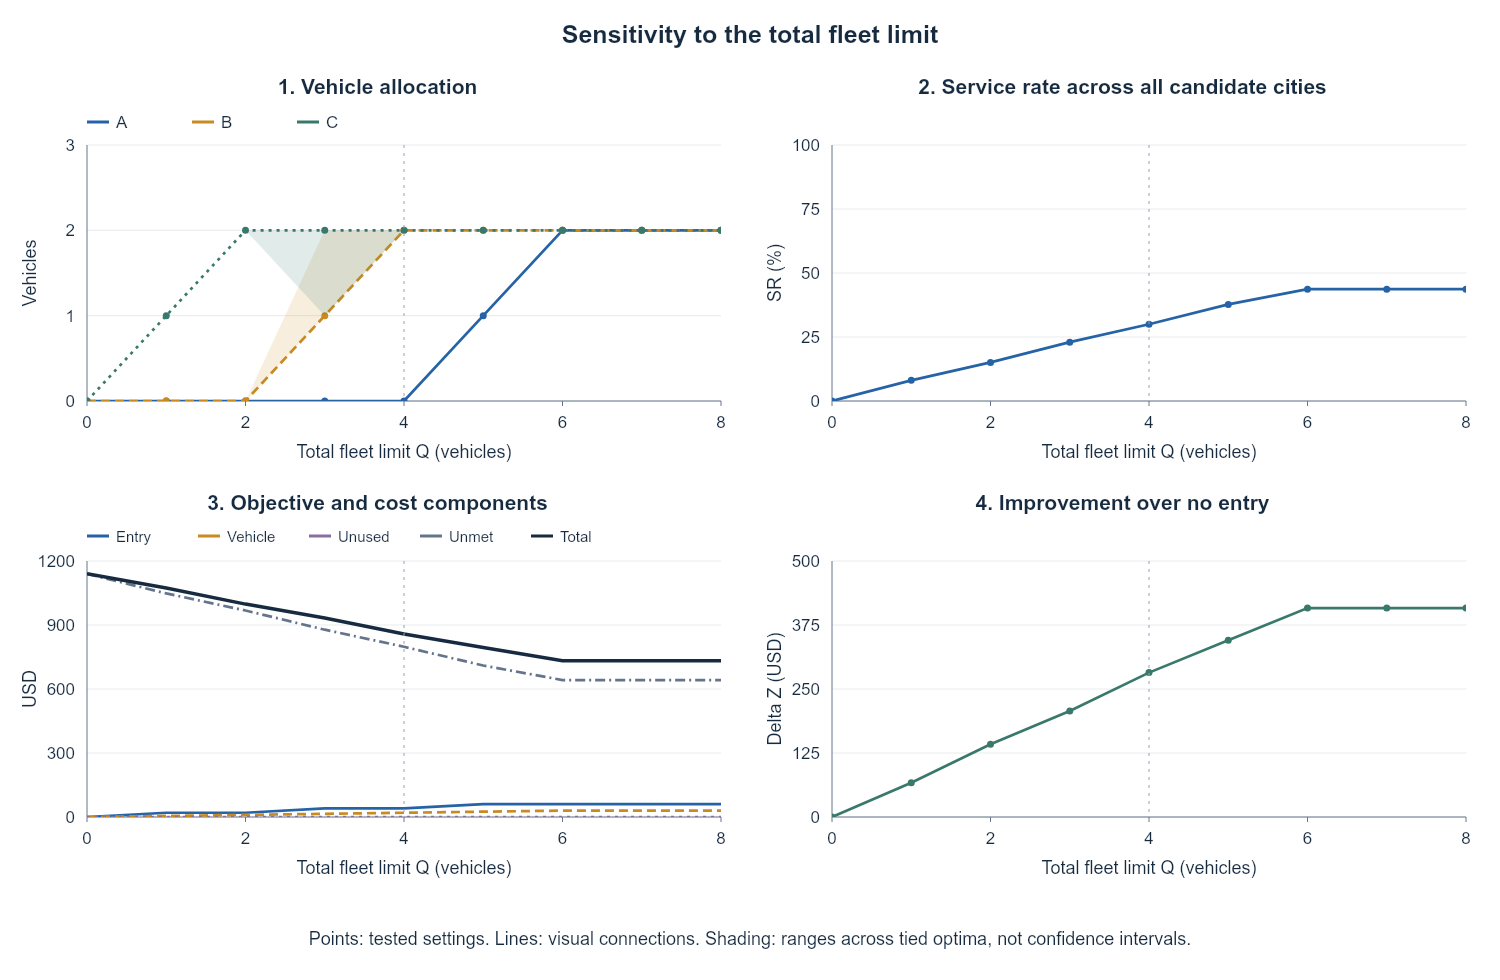
\includegraphics[width=\linewidth]{figures/smallcase/05_Q.png}
\caption{Allocation, service rate, cost, and improvement as the total fleet limit varies.}\label{fig:sc-05_Q}
\end{figure}
\textbf{Interpretation.} Increasing $Q$ from 4 to 5 adds one vehicle in A and increases the improvement by 63. Results remain unchanged for $Q\ge6$ because the city-specific limits sum to six vehicles. This insensitivity reflects deployment limits, not sufficient service of demand. At $Q=3$, allocations $(0,1,2)$ and $(0,2,1)$ are tied.

\subsubsection{Common Entry Cost $F$}
\begin{table}[H]
\centering\small
\caption{Selected Results: Common Entry Cost (Throughput in Trips/Year; Costs in USD)}\label{tab:sc-selected-F}
\begin{tabular}{lrrrrr}
\toprule
Value & $q^{\mathrm{rep}}$ & $\bar T$ & $\mathrm{SR}$ (\%) & $Z$ & $\Delta Z$\\\midrule
0 & $(1,1,2)$ & 35 & 30.7 & 810 & 330\\
8 & $(0,2,2)$ & 34.2 & 30 & 834 & 306\\
20 & $(0,2,2)$ & 34.2 & 30 & 858 & 282\\
160 & $(0,0,2)$ & 17.2 & 15.09 & 1,138 & 2\\
162 & $(0,0,0)$ & 0 & 0 & 1,140 & 0\\
200 & $(0,0,0)$ & 0 & 0 & 1,140 & 0\\
\bottomrule
\end{tabular}
\end{table}
\begin{figure}[H]
\centering
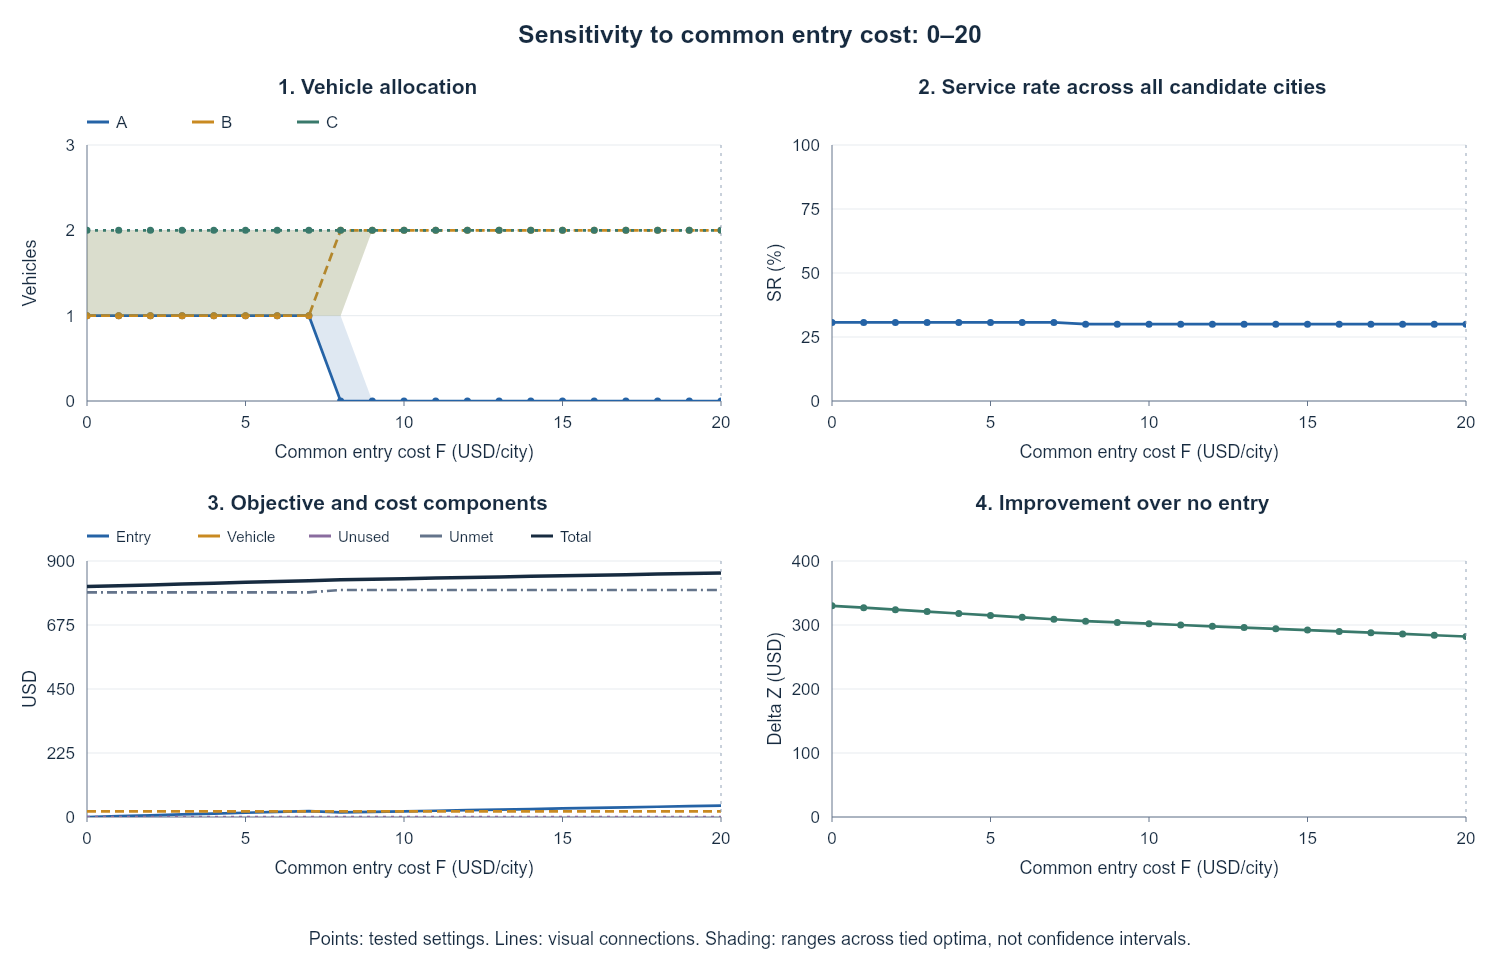
\includegraphics[width=\linewidth]{figures/smallcase/06_F_zoom.png}
\caption{Switch between concentrated and dispersed allocations for entry costs from 0 to 20.}\label{fig:sc-06_F_zoom}
\end{figure}
\begin{figure}[H]
\centering
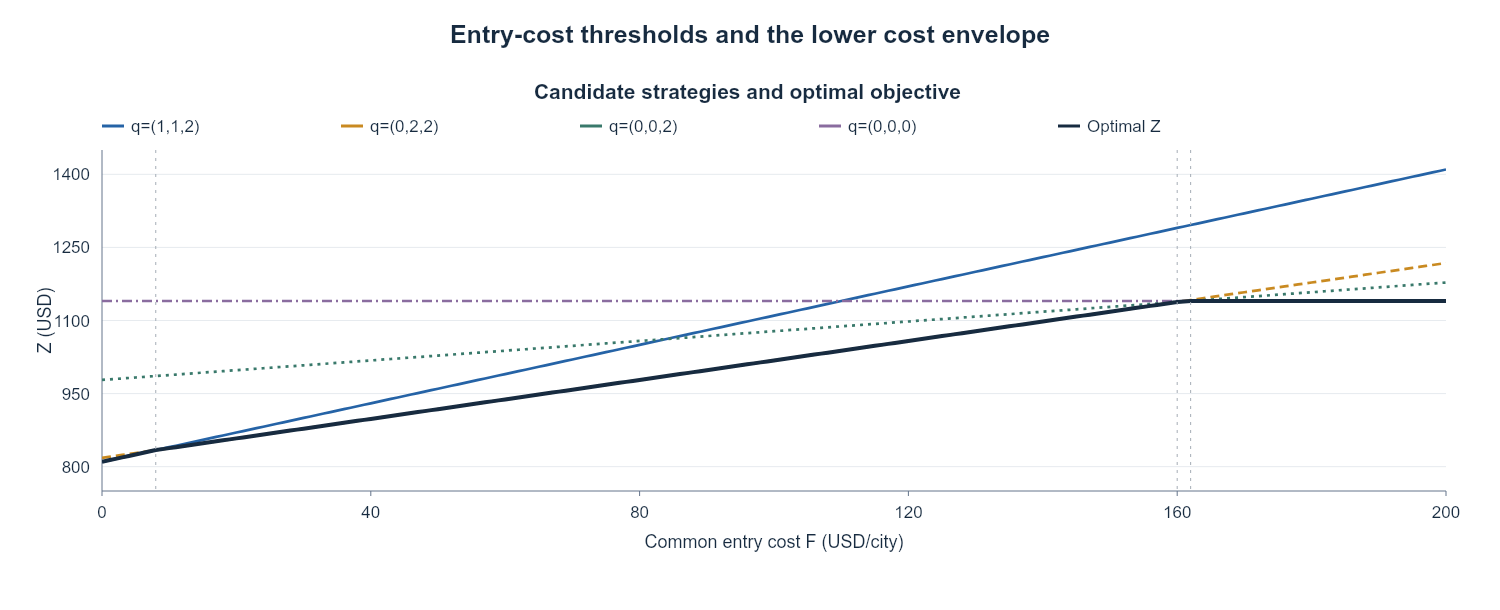
\includegraphics[width=\linewidth]{figures/smallcase/07_F_full.png}
\caption{Cost comparison showing switches to single-city entry and no entry at higher entry costs.}\label{fig:sc-07_F_full}
\end{figure}
\textbf{Interpretation.} When entry costs are low, the additional service from entering all three cities is worthwhile. The two-city allocation costs $818+2F$, while the three-city allocation costs $810+3F$; they tie at $F=8$. The lower envelope of all candidate cost functions selects three cities for $F<8$, B and C for $8<F<160$, C alone for $160<F<162$, and no entry for $F>162$. Adjacent strategies tie at the boundaries. These switching points apply to the current synthetic inputs.

\clearpage
\subsubsection{Vehicle Productivity $\kappa$}
\begin{table}[H]
\centering\small
\caption{Selected Results: Vehicle Productivity (Throughput in Trips/Year; Costs in USD)}\label{tab:sc-selected-kappa}
\begin{tabular}{lrrrrr}
\toprule
Value & $q^{\mathrm{rep}}$ & $\bar T$ & $\mathrm{SR}$ (\%) & $Z$ & $\Delta Z$\\\midrule
5 & $(0,2,2)$ & 18.2 & 15.96 & 1,018 & 122\\
10 & $(0,2,2)$ & 34.2 & 30 & 858 & 282\\
12 & $(0,2,2)$ & 39.4 & 34.56 & 806 & 334\\
12.5 & $(1,1,2)$ & 42.7 & 37.46 & 793 & 347\\
20 & $(1,1,2)$ & 61 & 53.51 & 610 & 530\\
\bottomrule
\end{tabular}
\end{table}
\begin{figure}[H]
\centering
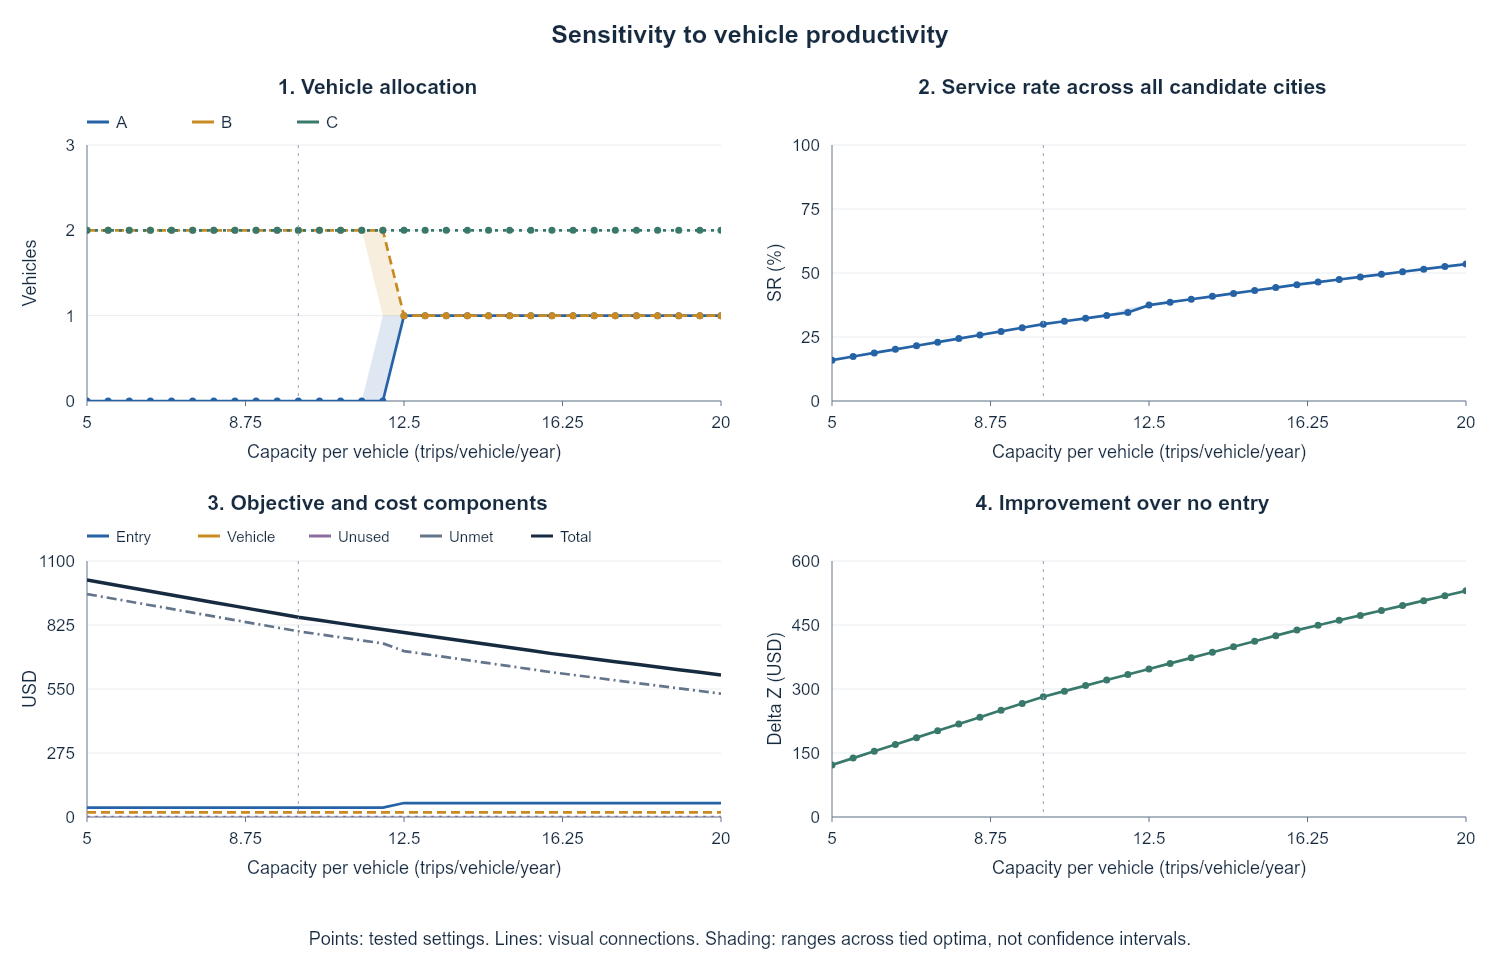
\includegraphics[width=\linewidth]{figures/smallcase/08_kappa.png}
\caption{Results from varying service capacity per vehicle.}\label{fig:sc-08_kappa}
\end{figure}
\textbf{Interpretation.} As productivity increases, the service provided by the first vehicle in A can become more valuable than that provided by the second vehicle in B. Concentrated and dispersed allocations tie at $\kappa=12$, while a three-city allocation is selected at 12.5. At $\kappa=20$, the representative allocation is $(1,1,2)$, the service rate is approximately 53.5\%, and the objective is 610. Unused capacity may increase relative to the baseline while throughput also rises, so unused capacity alone is not a sufficient performance measure.

\clearpage
\subsubsection{Market Size of A: $M_A$}
\begin{table}[H]
\centering\small
\caption{Selected Results: A's Market-Size Multiplier (Throughput in Trips/Year; Costs in USD)}\label{tab:sc-selected-M_A-multiplier}
\begin{tabular}{lrrrrr}
\toprule
Value & $q^{\mathrm{rep}}$ & $\bar T$ & $\mathrm{SR}$ (\%) & $Z$ & $\Delta Z$\\\midrule
0.5 & $(0,2,2)$ & 34.2 & 34.62 & 706 & 282\\
1 & $(0,2,2)$ & 34.2 & 30 & 858 & 282\\
1.25 & $(0,2,2)$ & 34.2 & 28.13 & 934 & 282\\
1.3 & $(2,0,2)$ & 34.24 & 27.81 & 948.8 & 282.4\\
2 & $(2,0,2)$ & 34.8 & 24.1 & 1,156 & 288\\
\bottomrule
\end{tabular}
\end{table}
\begin{figure}[H]
\centering
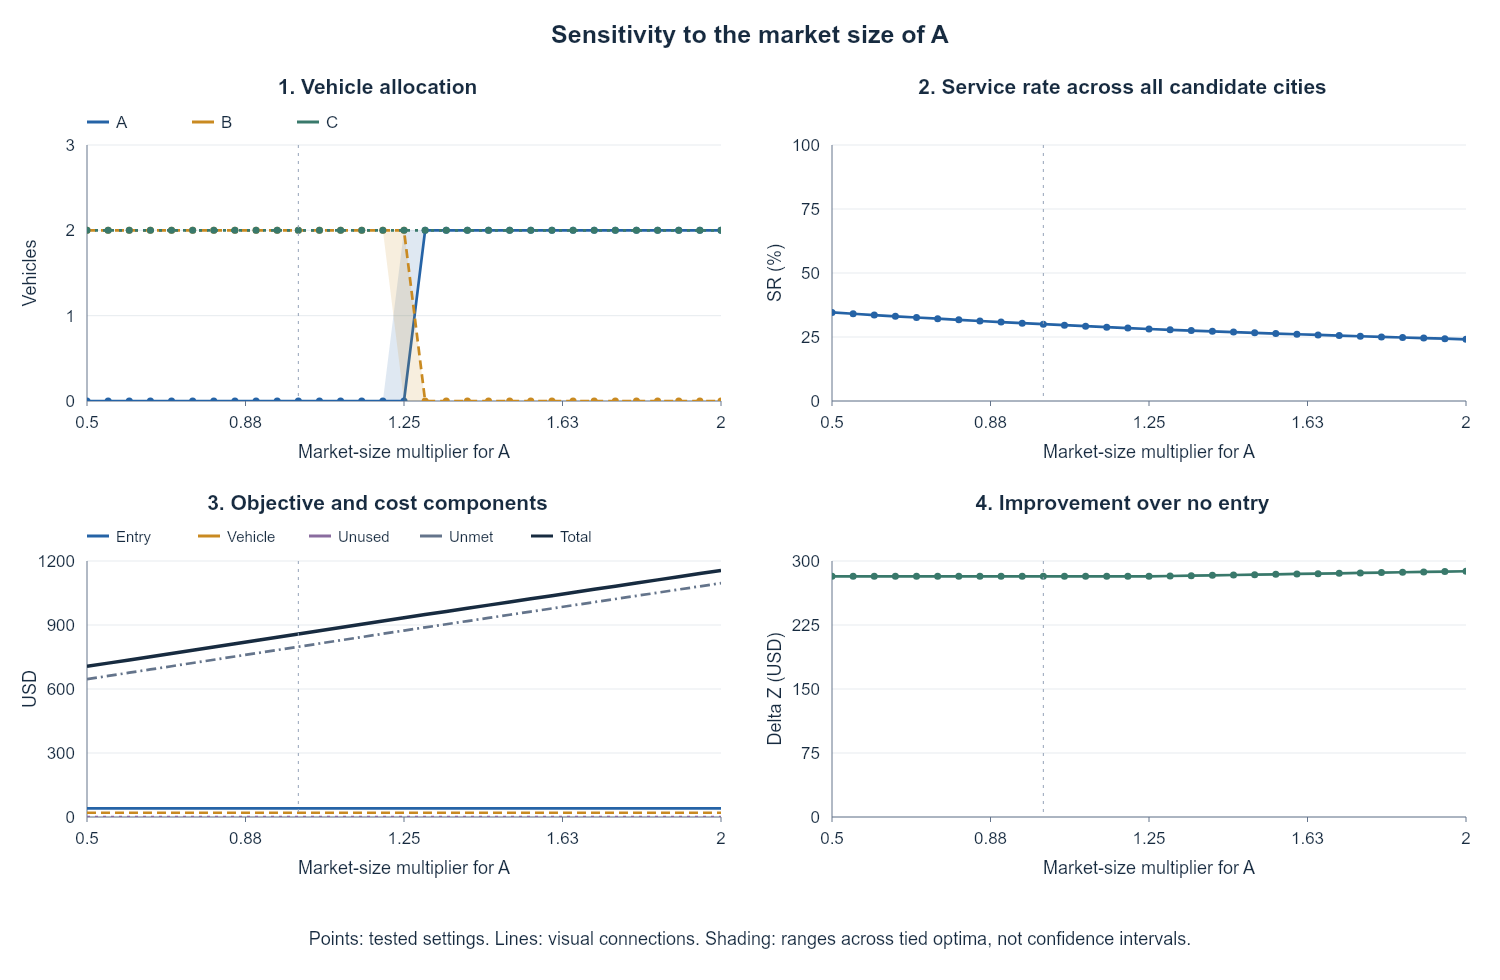
\includegraphics[width=\linewidth]{figures/smallcase/09_A_market.png}
\caption{Results from varying only A's market size. A multiplier of 1 corresponds to $M_A=80$.}\label{fig:sc-09_A_market}
\end{figure}
\textbf{Interpretation.} At a multiplier of 1.25 ($M_A=100$), allocations $(0,2,2)$ and $(2,0,2)$ tie. At 1.30 ($M_A=104$), allocation $(2,0,2)$ is selected, shifting B's two vehicles to A. When A and B have the same market size, their identical marginal choice-probability distributions imply equal expected throughput for the same number of vehicles. Increasing $M_A$ increases both mean demand and the magnitude of demand variation.

\clearpage
\subsubsection{Common Unused-Capacity Penalty $c^+$}
Because the baseline value is zero, the coefficient is increased from zero to positive values rather than decreased below zero. This experiment imposes an additional cost on unused capacity beyond the vehicle cost $K$.
\begin{table}[H]
\centering\small
\caption{Selected Results: Common Unused-Capacity Penalty (Throughput in Trips/Year; Costs in USD)}\label{tab:sc-selected-c_plus}
\begin{tabular}{lrrrrr}
\toprule
Value & $q^{\mathrm{rep}}$ & $\bar T$ & $\mathrm{SR}$ (\%) & $Z$ & $\Delta Z$\\\midrule
0 & $(0,2,2)$ & 34.2 & 30 & 858 & 282\\
5 & $(0,2,2)$ & 34.2 & 30 & 887 & 253\\
10 & $(0,2,2)$ & 34.2 & 30 & 916 & 224\\
15 & $(0,2,2)$ & 34.2 & 30 & 945 & 195\\
15.5 & $(1,1,2)$ & 35 & 30.7 & 947.5 & 192.5\\
20 & $(1,1,2)$ & 35 & 30.7 & 970 & 170\\
\bottomrule
\end{tabular}
\end{table}
\begin{figure}[H]
\centering
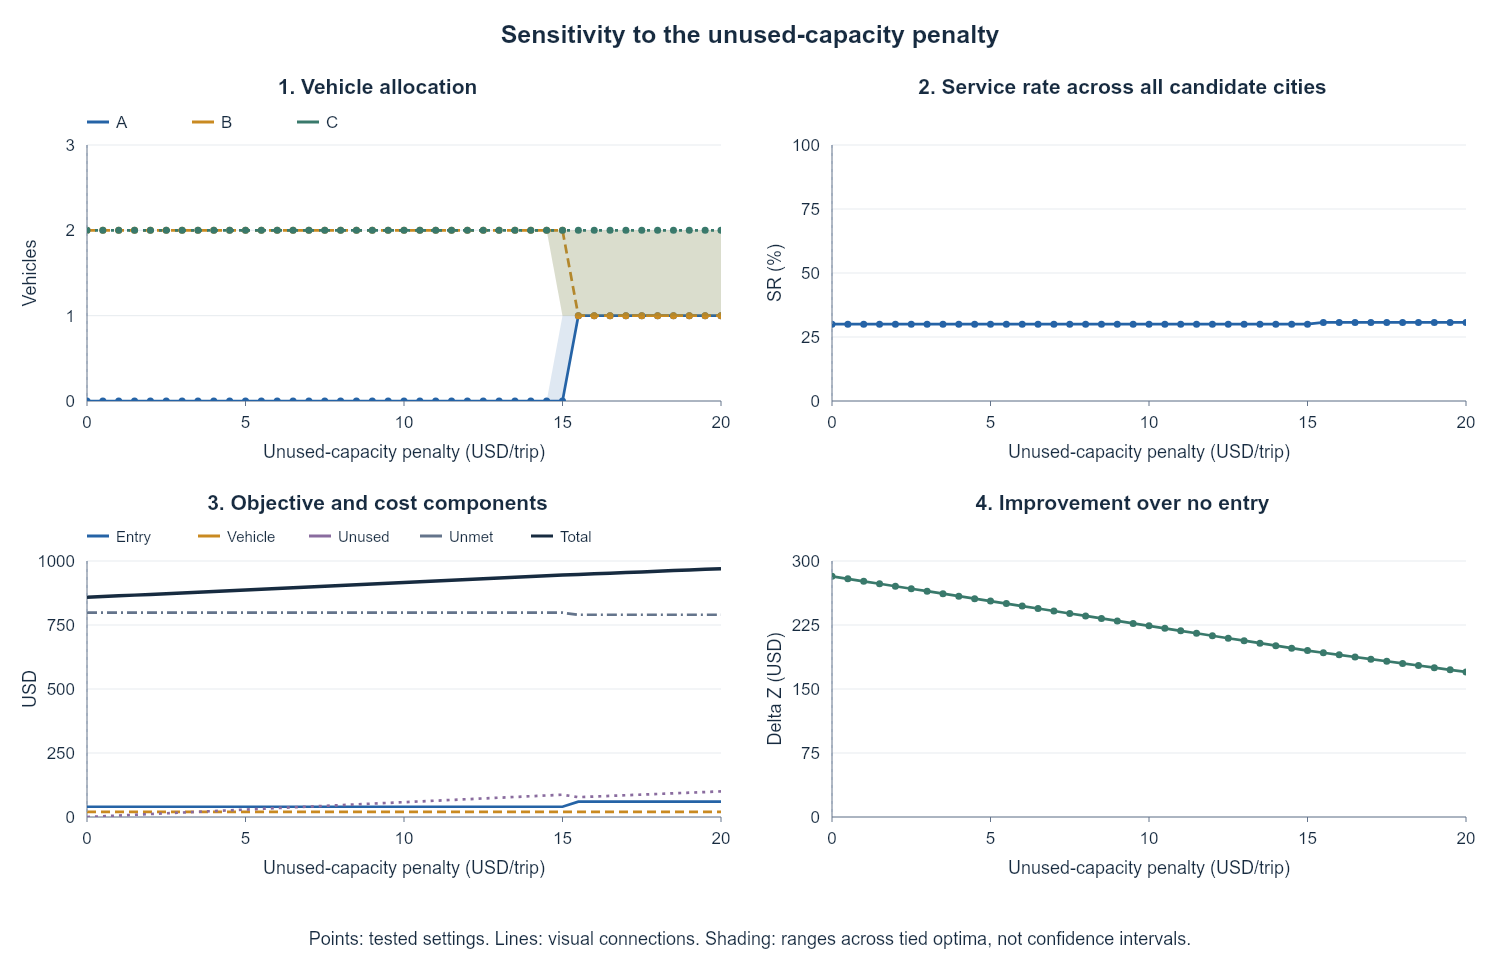
\includegraphics[width=\linewidth]{figures/smallcase/13_cplus.png}
\caption{Sensitivity of allocations and performance to the unused-capacity penalty.}\label{fig:sc-13_cplus}
\end{figure}
\textbf{Interpretation.} At the tested values from 0 to 14.5, allocation $(0,2,2)$ remains optimal while its cost increases. Its average unused capacity is 5.8 trips, giving $Z=858+5.8c^+$. The dispersed allocations $(1,1,2)$ and $(1,2,1)$ have unused capacity of 5 trips and cost $Z=870+5c^+$. The two cost expressions are equal at $c^+=15$, where all three allocations tie. At the tested values from 15.5 to 20, the two dispersed allocations are optimal. Following the switch, the service rate increases from 30.0\% to approximately 30.70\%, but the added unused-capacity cost reduces the improvement at $c^+=20$ to 170, below the baseline value of 282.

\clearpage
\subsubsection{Demand Variability $\alpha$ with Fixed Mean Demand}
\[
\bar p_c=\frac{1}{|S|}\sum_{s\in S}p_c^s,\qquad
p_c^s(\alpha)=\bar p_c+\alpha(p_c^s-\bar p_c),\quad 0\le\alpha\le1.
\]
At $\alpha=0$, every scenario equals mean demand; $\alpha=1$ recovers the original scenarios. Only the magnitude of variation in the existing scenarios is adjusted; no new random scenarios are sampled.
\begin{table}[H]
\centering\small
\caption{Selected Results: Demand Variability (Throughput in Trips/Year; Costs in USD)}\label{tab:sc-selected-alpha}
\begin{tabular}{lrrrrr}
\toprule
Value & $q^{\mathrm{rep}}$ & $\bar T$ & $\mathrm{SR}$ (\%) & $Z$ & $\Delta Z$\\\midrule
0 & $(0,2,2)$ & 40 & 35.09 & 800 & 340\\
0.35 & $(0,2,2)$ & 40 & 35.09 & 800 & 340\\
0.4 & $(0,2,2)$ & 40 & 35.09 & 800 & 340\\
0.5 & $(0,2,2)$ & 40 & 35.09 & 800 & 340\\
1 & $(0,2,2)$ & 34.2 & 30 & 858 & 282\\
\bottomrule
\end{tabular}
\end{table}
\begin{figure}[H]
\centering
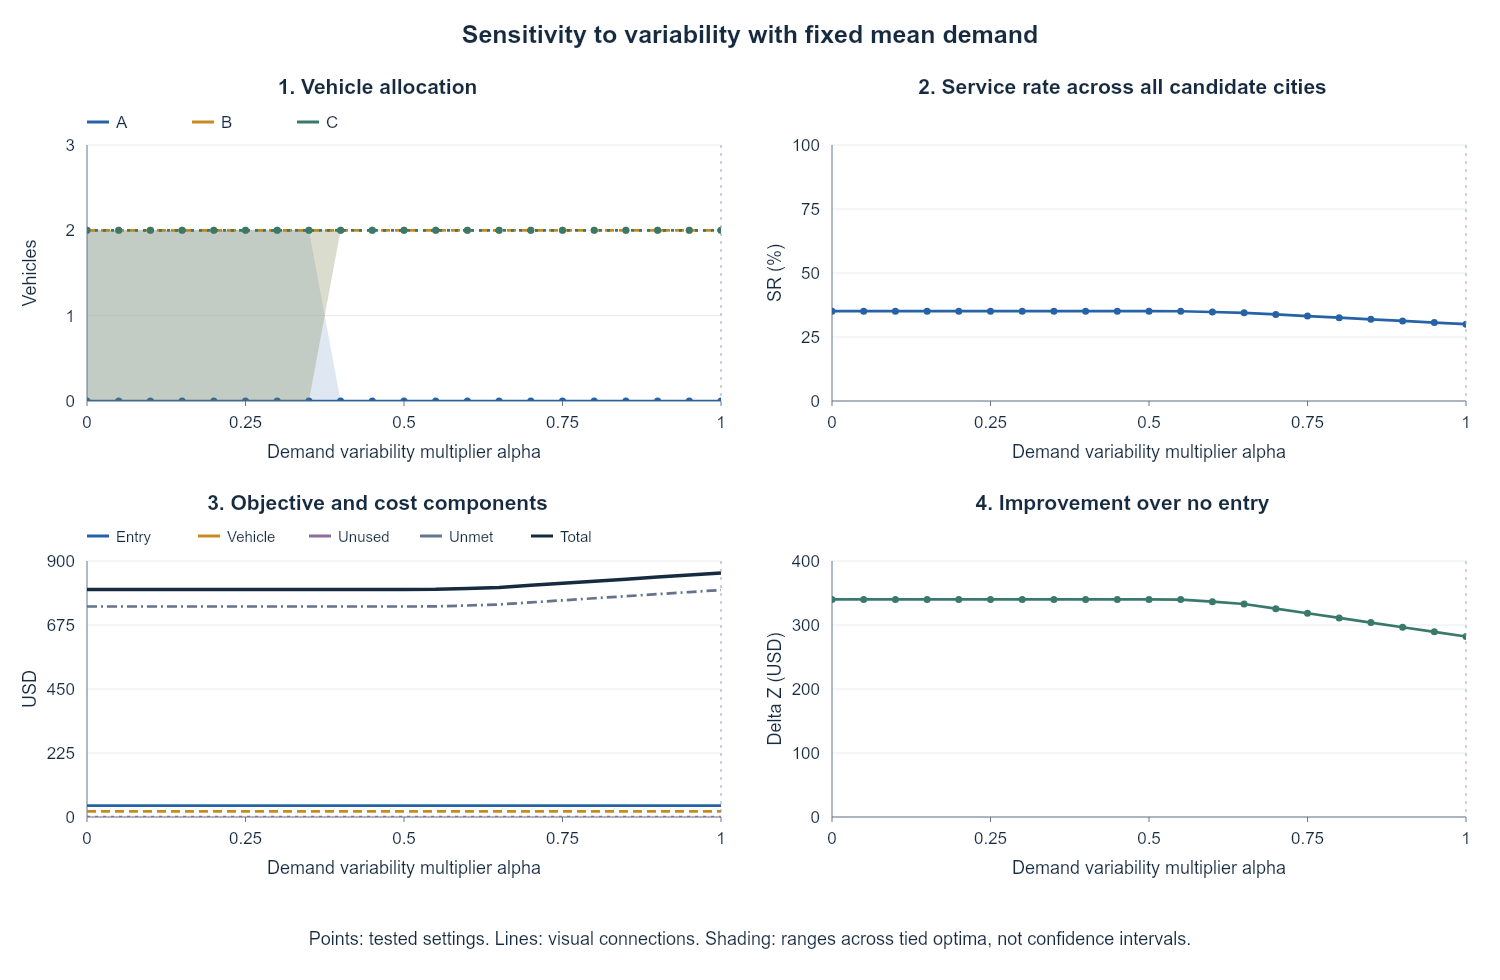
\includegraphics[width=\linewidth]{figures/smallcase/10_alpha.png}
\caption{Results from varying demand variability while preserving mean demand.}\label{fig:sc-10_alpha}
\end{figure}
\textbf{Interpretation.} Without demand variation, allocations $(0,2,2)$, $(2,0,2)$, and $(2,2,0)$ tie. Under the original variability, only $(0,2,2)$ is optimal, and the objective increases from 800 to 858. The set of tied optima and performance can change even when the representative allocation is unchanged, so a single representative allocation is insufficient to establish insensitivity.

\clearpage

\subsubsection{Three-Level Checks of the Other Main Inputs}
Alongside the switching-point analysis, the original three-level experiments for eight inputs are retained. The $M$ multiplier applies to all three cities, as do the other common parameter levels except the system-wide limit $Q$. Inputs not listed in a row remain at their baseline values. Units follow the input table, except that $M$ is expressed as a multiplier.
\begin{table}[H]
\centering\small
\caption{Three-Level Checks of Eight Inputs: Representative Allocations and Performance}\label{tab:sc-original24}
\begin{tabular}{lrrrrr}
\toprule
Parameter & Value & $q^{\mathrm{rep}}$ & $\mathrm{SR}$ (\%) & $Z$ & $\Delta Z$\\\midrule
$M/M^{\mathrm{base}}$ & 0 & $(0,0,0)$ & --- & 0 & 0\\
$M/M^{\mathrm{base}}$ & 1 & $(0,2,2)$ & 30 & 858 & 282\\
$M/M^{\mathrm{base}}$ & 2 & $(0,2,2)$ & 15.96 & 1,976 & 304\\
$\kappa$ & 5 & $(0,2,2)$ & 15.96 & 1,018 & 122\\
$\kappa$ & 10 & $(0,2,2)$ & 30 & 858 & 282\\
$\kappa$ & 20 & $(1,1,2)$ & 53.51 & 610 & 530\\
$\bar q$ & 0 & $(0,0,0)$ & 0 & 1,140 & 0\\
$\bar q$ & 2 & $(0,2,2)$ & 30 & 858 & 282\\
$\bar q$ & 4 & $(0,2,2)$ & 30 & 858 & 282\\
$Q$ & 0 & $(0,0,0)$ & 0 & 1,140 & 0\\
$Q$ & 4 & $(0,2,2)$ & 30 & 858 & 282\\
$Q$ & 8 & $(2,2,2)$ & 43.68 & 732 & 408\\
$F$ & 0 & $(1,1,2)$ & 30.7 & 810 & 330\\
$F$ & 20 & $(0,2,2)$ & 30 & 858 & 282\\
$F$ & 1,000 & $(0,0,0)$ & 0 & 1,140 & 0\\
$K$ & 0 & $(0,2,2)$ & 30 & 838 & 302\\
$K$ & 5 & $(0,2,2)$ & 30 & 858 & 282\\
$K$ & 100 & $(0,0,0)$ & 0 & 1,140 & 0\\
$c^+$ & 0 & $(0,2,2)$ & 30 & 858 & 282\\
$c^+$ & 2 & $(0,2,2)$ & 30 & 869.6 & 270.4\\
$c^+$ & 5 & $(0,2,2)$ & 30 & 887 & 253\\
$c^-$ & 0 & $(0,0,0)$ & 0 & 0 & 0\\
$c^-$ & 10 & $(0,2,2)$ & 30 & 858 & 282\\
$c^-$ & 20 & $(0,2,2)$ & 30 & 1,656 & 624\\
\bottomrule
\end{tabular}
\end{table}
\begin{figure}[H]
\centering
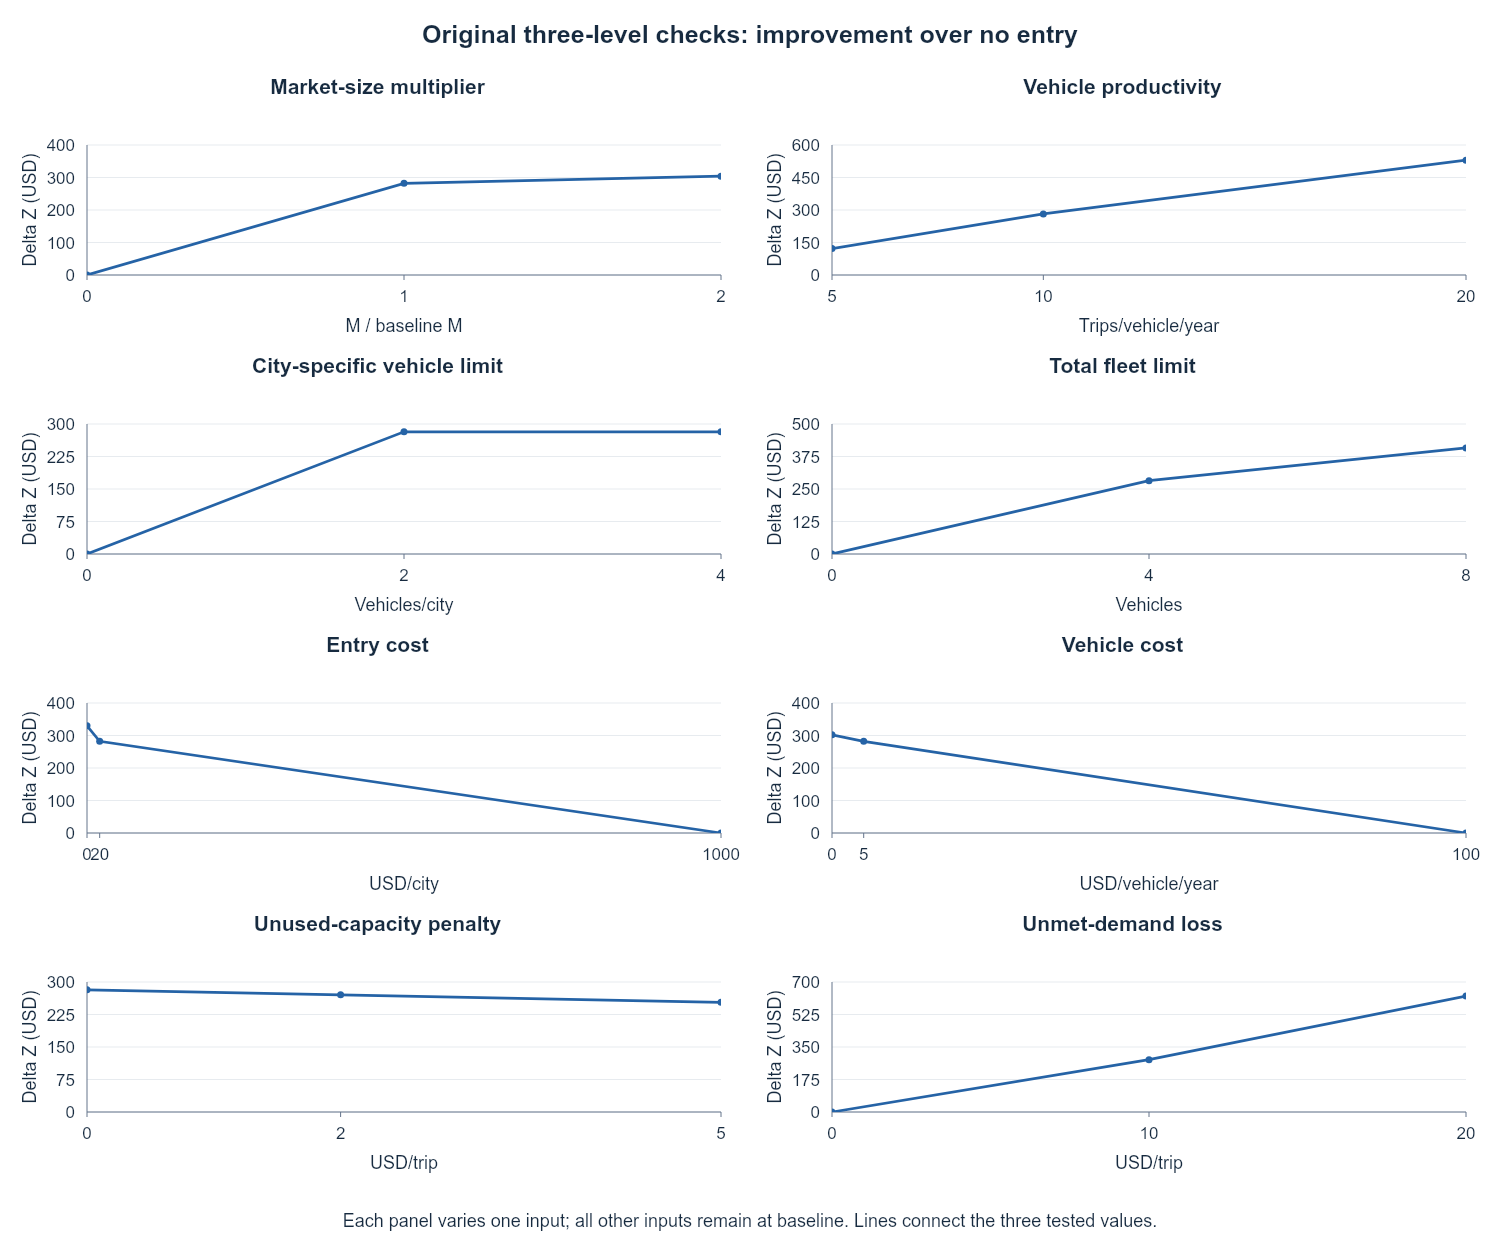
\includegraphics[width=\linewidth]{figures/smallcase/12_original_sweeps.png}
\caption{Improvement over no entry for the original 24 settings. This figure alone does not establish exact switching points between the three tested levels.}\label{fig:sc-12_original_sweeps}
\end{figure}
\textbf{Interpretation.} Doubling $M$ increases the objective, but also increases the improvement from 282 to 304. Relaxing each city's vehicle limit from two to four does not change the optimal cost under baseline conditions. No entry is optimal at $K=100$. At $c^-=20$, unmet demand receives a higher monetary valuation even though the allocation is unchanged. Testing only $c^+=0,2,5$ yields no allocation change, whereas the expanded experiment identifies a switching point at 15. Any claim of insensitivity must therefore state the range examined.


\end{document}
